\documentclass[linenumbers, twocolumn]{aastex631}


\newcommand{\vdag}{(v)^\dagger}
\newcommand\aastex{AAS\TeX}
\newcommand\latex{La\TeX}

\begin{document}

\title{The Milky Way and M31 Halo Remnant Shape}



\author[0000-0002-2527-8899]{Mika Lambert}
\affiliation{Steward Observatory and Department of Astronomy, University of Arizona, 933 N. Cherry Ave., Tucson, AZ 85721, USA}


%\begin{abstract}

%This example manuscript is intended to serve as a tutorial and template for authors to use when writing their own AAS Journal articles. The manuscript includes a history of \aastex\ and includes figure and table examples to illustrate these features. Information on features not explicitly mentioned in the article can be viewed in the manuscript comments or more extensive online documentation. Authors are welcome replace the text, tables, figures, and bibliography with their own and submit the resulting manuscript to the AAS Journals peer review system.  The first lesson in the tutorial is to remind authors that the AAS Journals, the Astrophysical Journal (ApJ), the Astrophysical Journal Letters (ApJL), the Astronomical Journal (AJ), and the Planetary Science Journal (PSJ) all have a 250 word limit for the abstract\footnote{Abstracts for Research Notes of the American Astronomical  Society (RNAAS) are limited to 150 words}.  If you exceed this length the Editorial office will ask you to shorten it. This abstract has 161 words.

%\end{abstract}

%% Keywords should appear after the \end{abstract} command. 
%% The AAS Journals now uses Unified Astronomy Thesaurus concepts:
%% https://astrothesaurus.org
%% You will be asked to selected these concepts during the submission process
%% but this old "keyword" functionality is maintained in case authors want
%% to include these concepts in their preprints.
%\keywords{Milky Way,  M31, Dark Matter Halo} 

\section{Introduction} \label{sec:intro}

%\subsection{Proposed Topic}
The two most massive bodies in the Local Group (LG) are the MW and M31.
Many simulations have been conducted predicting the motions of the Milky Way (MW) and Andromeda Galaxy (M31) and their course to a future collision \citep{2012VanDerMarel}.
We propose investigating the characteristics of the dark matter halo remnant due to this future merger of the MW and M31. 
Using N-body simulations, we will explore the density profile of the halo remnant and the 3-dimensional shape of the halo. 

%\subsection{Why this topic matters to our understanding of galaxy evolution}
As M31 is the closest galaxy to the MW, our knowledge of that galaxy is greater than most other bodies in the universe. 
N-body simulations of the merger event between the MW and M31 have accelerated our understanding of galactic merger events which have been hypothesized to be the source of the formation of high-mass elliptical galaxies. 
Understanding the profile of the halo remnant will further aid our quest to understand the behavior of cold dark matter. 
The resulting density profile from our experiment could also be compared to galaxies in more clustered environments that are believed to be the result of mergers which would shed light on the differences between mergers in the field versus in dense environments.
Further research could also be done on higher redshift galaxies (z $>$ 1) to look at early galaxy formation and merging.

%\subsection{Our current understanding of the topic}

According to \cite{2012VanDerMarel} the next major cosmic event to happen in the Local Group (LG) is the merger of the MW and M31 in $\sim$ 5 Gyrs. 
This event will not only change the physical shape of the baryonic matter of the LG, but also the dark matter halos of the galaxies.
We currently know that for equal-mass mergers, the shape of the halo remnant is dependent on the way the galaxies merge because the merger axis dictates the elongation shape, and the size of the remnant is related to the total energy of the merger \citep{2019drakos}. 
Another interesting aspect of the halos is the concentration of dark matter.
Modeling the density distribution of dark matter halos of galaxies is well defined by the Navarro-Frenk-White (NFW) profile \citep{1996NFW}. Visualizing the density profile of the halos using contour lines shows us the concentration of dark matter as seen in Figure \ref{fig:drakos}.
Astronomers also use simple relations between the mass of a galaxy's halo and its stellar mass using abundance matching \citep{2018Wechsler}. Abundance matching is the assumption that the halo mass is directly correlated to the stellar mass.



%\subsection{Open questions in the field}
There are still many open questions within the realm of galaxy halo remnants.
More complex N-body simulations should be conducted accounting for the satellite galaxy's influence on the merging process. Also, the halos of dense galaxy clusters are still not well defined \citep{2019drakos}.
We can use these galaxy halos as laboratories for directly and indirectly detecting dark matter particles. An example of direct detection would be using our position in the MW to come across dark particles using facilities like LIGO, and indirect detection would search for the radiation produced by decaying dark matter particles \citep{2012Frenk_White}. In our own LG, the shape of the mass distribution of the merger remnant's halo would be an interesting question to pursue.
\begin{figure}[ht]
    \centering
    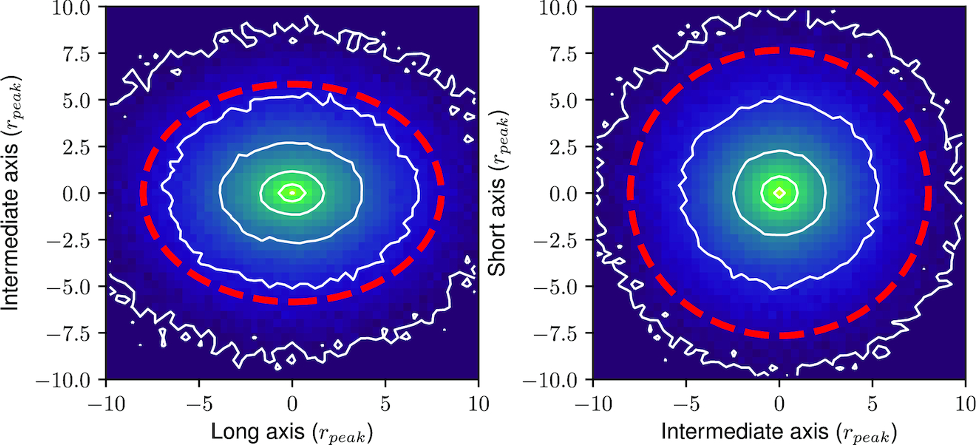
\includegraphics[scale=0.5]{drakos_fig_6.png}
    \caption{The density contours of the simulated remnant halos are in white, and the measured shape ratio is shown in red from \cite{2019drakos}.}
    \label{fig:drakos}
\end{figure}


\begin{figure*}
    \centering
    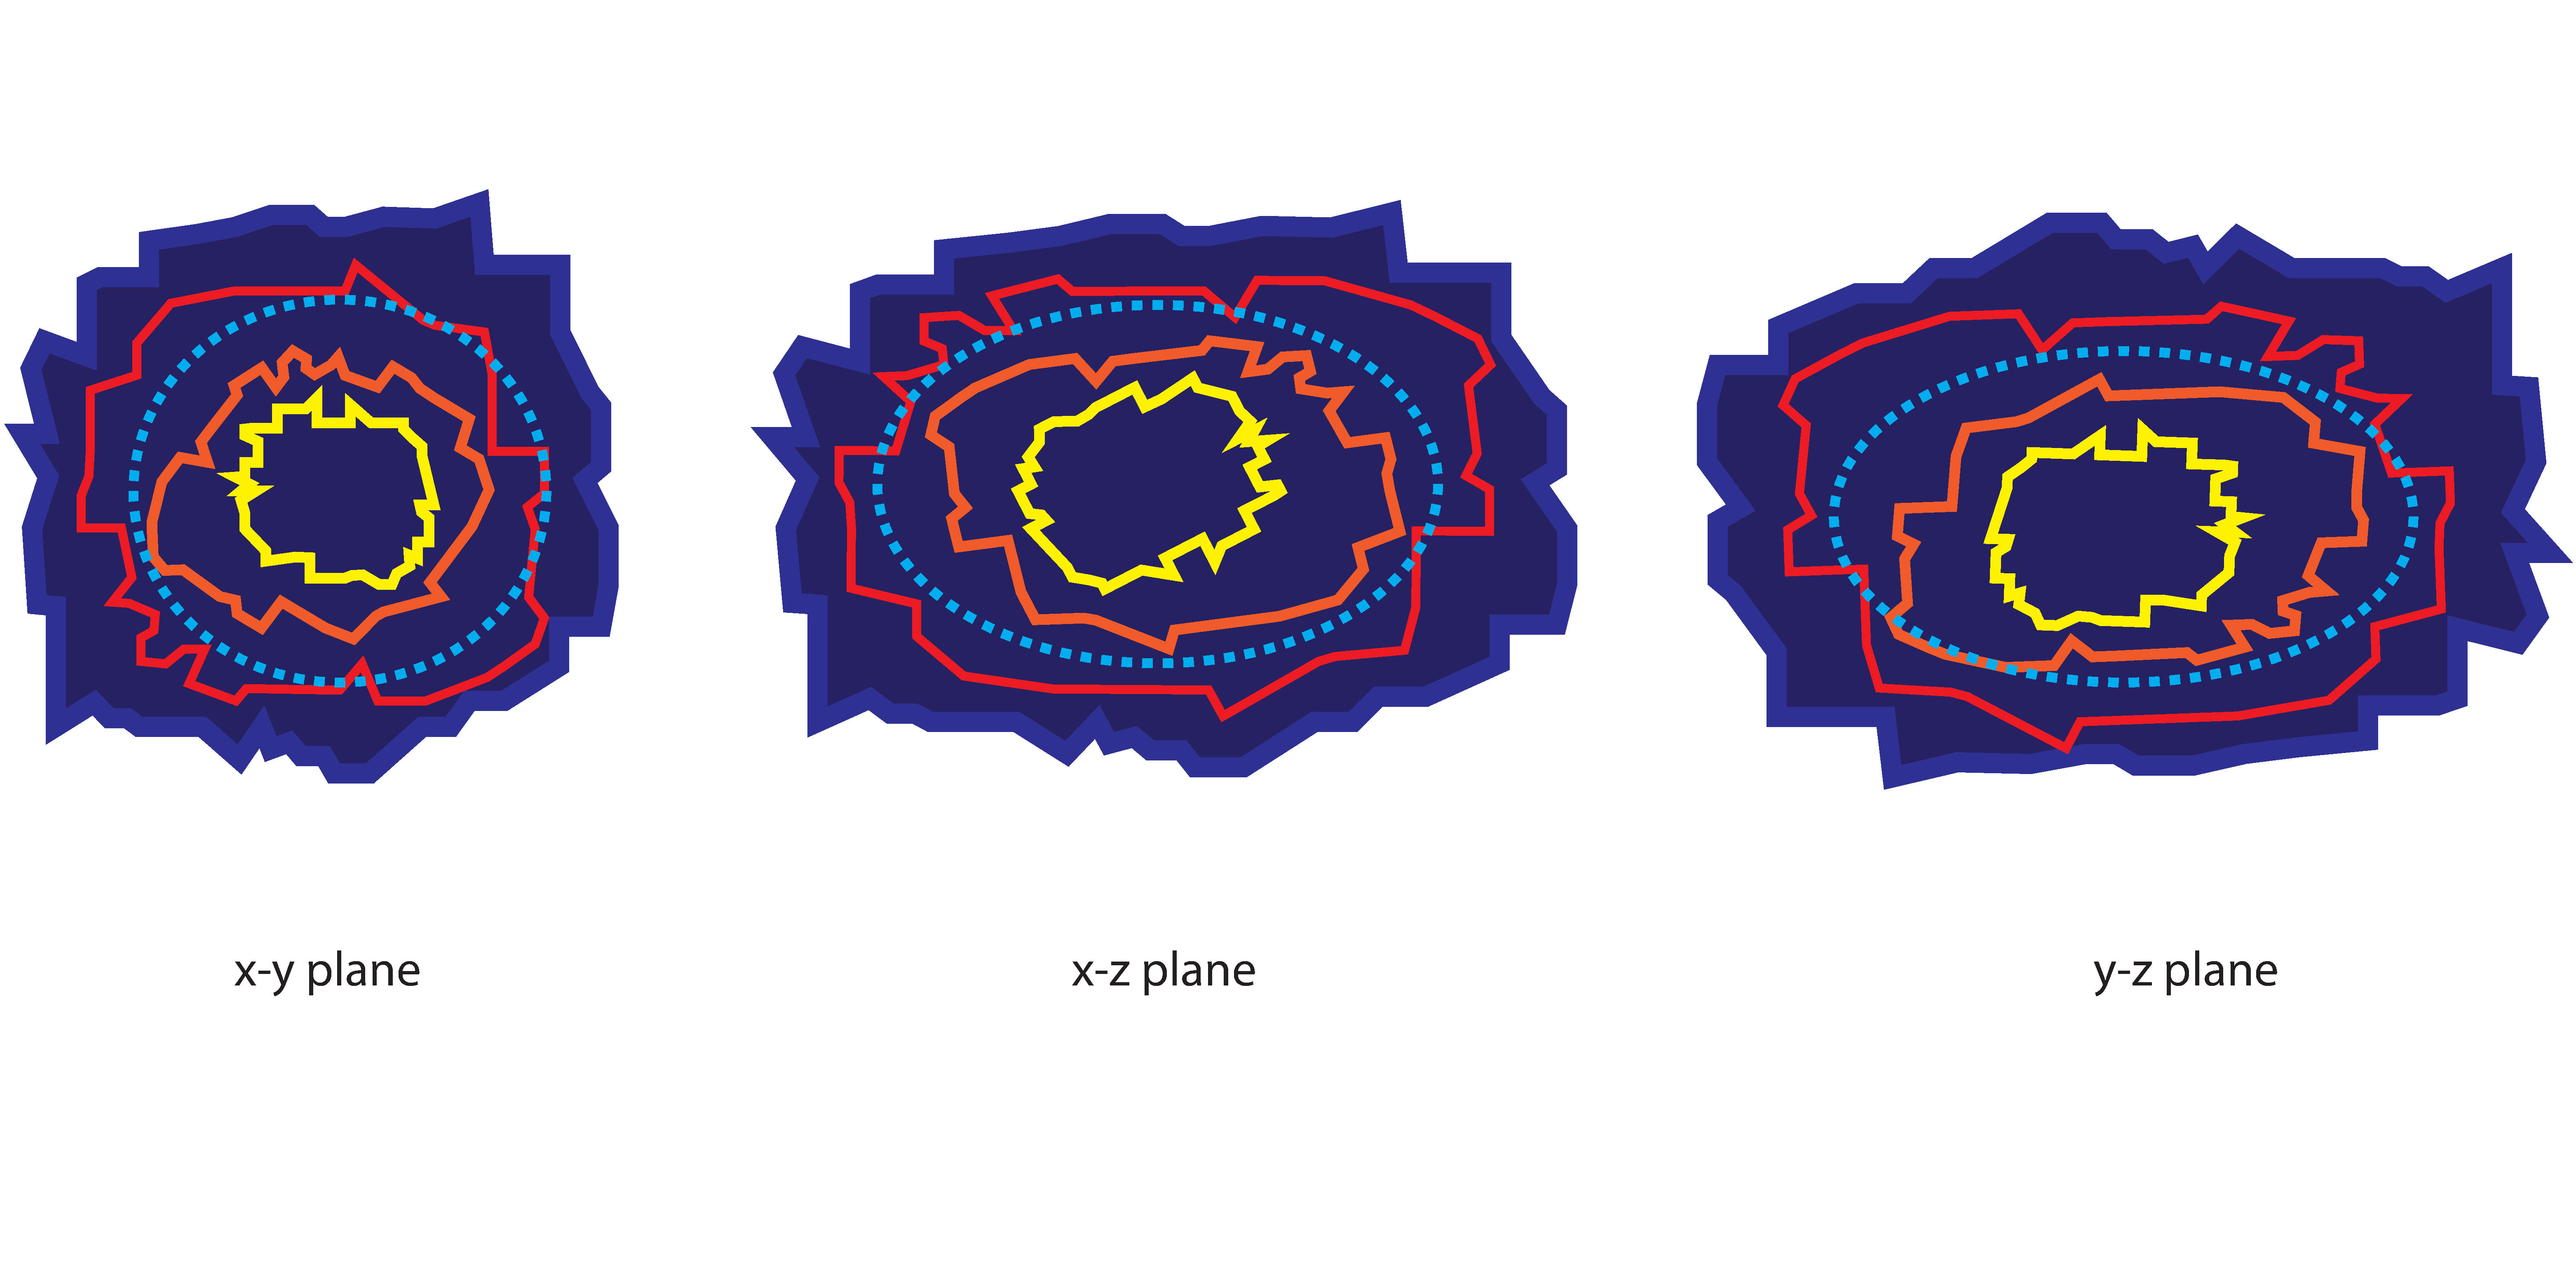
\includegraphics[width=\textwidth,height=10cm]{ASTR400B_proposal_diagram_2.pdf}
    \caption{The expected results from our methodology. Left: The dark matter halo of the MW before merger with density contours at 1$\sigma$ (yellow), 2$\sigma$ (orange), and 3$\sigma$ (red). Right: The halo remnant from the MW-M31 merger. We see that the shape is prolate compared to the original MW halo. The blue dashed line represents the ellipse with a projected axis ratio that appears to fit the halo distribution.}
    \label{fig:method_fig}
\end{figure*}

\section{Proposal} \label{sec:proposal}



\subsection{Questions} \label{sec:questions}
We will be investigating the change in the 3-dimensional shape of the dark matter distribution from the MW halo to the merger remnant halo. 
Looking at the different axes of the distribution, We will determine whether the halo is spheroidal or elongated. 
We will describe the shape of the halo based on whether the shape is prolate, oblate, or triaxial which refer to the direction of flattening of the spheroidal objects.
We will also investigate the elliptical shape of the 2D projections of the halo in the three planes and characterize their semi-major and semi-minor axes.
%2. Is the 3D dark matter distribution spheroidal? or elongated like an ellipsoid? What do terms like prolate, oblate, or triaxial halos mean? https://astronomy.com/news/2010/ 01/astronomers-map-the-shape-of-galactic-dark-matter


\subsection{Approach} \label{sec:approach}
First, we will need to probe the shape of the spatial mass distribution of the MW halo at snapshot 0 using a 2D histogram along all three axes to investigate any non-spheroidal attributes it may have. To do this, we will implement the code from Lab 7 to create the density contours, and we will also need to rotate the position vectors so that the halo's angular momentum is aligned with the z-axis. We will look at the x-y plane, the x-z plane, and the y-z plane distributions for elongation.
We will then use visual checks to estimate the elliptical ratio of the semi-major and semi-minor axes in each triaxial direction.
The code we will create will use the $\tt{matplotlib}$ ellipse function and we will try different values for semi-major and semi-minor axes. 

Then, we will do a similar procedure for the MW-M31 halo remnant using snapshot 700 using a 2D histogram along the three axes and look for prolate or oblate features by looking at the x-y plane, the x-z plane, and the y-z plane. We use snapshot 700 because the conversion from snapshot to years is Snapshot$*10/.7$ = time (Myrs), therefore a snapshot value of 700 gives a time of 10Gyrs. This is where we define the merging galaxies to be relaxed dynamically, and the stars from the MW and M31 are well mixed according to \cite{2012VanDerMarel}. If only one of the planes shows elongation, we will assume the shape is more oblate. If two of the planes show elongation, we will assume the distribution is more prolate. If all three planes are relatively circular, then we will assume the halo remnant distribution is spheroidal. If we see that the axes are different in all three planes we will assume the shape is triaxial. We will also estimate the ellipsoidal measurement of the semi-major and semi-minor axes for the remnant.

%If feasible, we would also like to plot the positional distribution of the remnant in a 3D plot using $\tt{matplotlib}$.

%what are we defining as remnant - when the system is relaxed and the stars from MW and M31 are well mixed. According to Besla (2012) this would be equivalent to 10 Gyrs or snapshot 700 (snapshot..num *10/.7)
% axis ratio code: 


\subsection{Methodology} \label{sec:method}



The density contours seen in Figure \ref{fig:method_fig} show how concentrated the mass of the halo is. The blue line is the estimated projected ellipse for the corresponding plane. We will use visual checks to determine what the estimated axis ratio is.


\subsection{Hypothesis} \label{sec:hypothesis}
As seen in Figure \ref{fig:drakos} for the merger between two equal-mass galaxies, we would expect a similar shape to emerge from the halo of the MW-M31 halo remnant which is more triaxial than spheroidal with one long axis and two short axes as seen in Figure \ref{fig:method_fig}. 
This makes sense due to the momentum the collision transfers and we would expect the axis of elongation would be in the direction of relative motion between the galaxies.
Prolateness also depends on the amount of mass loss, so we can use our result to estimate the amount of mass that would no longer be under the gravitational effects of the remnant.


\bibliography{sample631}{}
\bibliographystyle{aasjournal}

%% This command is needed to show the entire author+affiliation list when
%% the collaboration and author truncation commands are used.  It has to
%% go at the end of the manuscript.
%\allauthors

%% Include this line if you are using the \added, \replaced, \deleted
%% commands to see a summary list of all changes at the end of the article.
%\listofchanges

\end{document}

% End of file `sample631.tex'.
